\documentclass[aspectratio=169]{beamer}

%
% Choose how your presentation looks.
%
% For more themes, color themes and font themes, see:
% http://deic.uab.es/~iblanes/beamer_gallery/index_by_theme.html
%
\mode<presentation>
\mode<presentation>
{
  \usetheme{Ilmenau}      % or try Darmstadt, Madrid, Warsaw, ...
  \usecolortheme{beaver} % or try albatross, beaver, crane, ...
  \usefonttheme{default}  % or try serif, structurebold, ...
  \setbeamertemplate{navigation symbols}{}
  \setbeamertemplate{caption}[numbered]
} 
\usepackage[english]{babel}
\usepackage[utf8x]{inputenc}
\usepackage{graphicx}
\usepackage{setspace}
\usepackage{tikz} \usetikzlibrary{snakes}
\usepackage{epstopdf}
\usepackage[round]{natbib}

\usepackage[english]{babel}
\usepackage[utf8x]{inputenc}
\title[Power and responsibility]{Falling house prices hurt incumbents}
\author{Frederik G. Hjorth \and Martin Vinæs Larsen}
\institute[UCPH]{\large{Department of Political Science \\ University of Copenhagen}}
\date[May 2015]{CVAP seminar, May 2015}

\begin{document}
	
	\begin{frame}
		\titlepage
	\end{frame}
	
	
\section{Politicized homes?}

	\begin{frame}{Politicized homes}
	One of the key economic features of post industrial nations is mass home ownership.
	
	\vspace{0.2in}
	
	Home ownership is obviously an important variable when understanding contemporary politics.
	\begin{itemize}
		\item Home ownership is the main form of ``capital'' ordinary people have.
		\item One's homes is a key part of one's control over one's immediate context.
		\item Home ownership is often the  focus of political rhetoric.
	\end{itemize}
	
		\vspace{0.2in}
		
	Inspite of this relatively little research has focused on how home-ownership shapes political behavior.
		\end{frame}	
	
		\begin{frame}{Politicized homes}
		The few papers on housing have focused on how owning a home might affect preferences for social spending and, in turn, demand for right-wing parties. 	
						\vspace{0.2in}	
						
		In the present research we look at another way housing may influence political behavior; what might be called a ``personal grievance hypothesis''.
		
			\vspace{0.2in}	
			
		Namely, that you blame (or credit) governing politician for any personal grievance (favor) that you might experience as a home owner; specifically, whether your house price (appreciate) depreciates.
		
					\vspace{0.2in}	
					
				
			\end{frame}	
	\begin{frame}{House prices as a personal economic grievance}
		
	
		
	This is at odds with recieved wisdom on economic voting: ``The political consequences of economic conditions are not carried by personally experienced hardships. Rather, a citizen's political response to economic conditions is mediated by judgments that are collectively oriented.'' (Kinder Kiewiet, 1979)
	
	\vspace{0.2in}
	
	However, the consequences of personal economic hardships has primarily been explored through (1) perception of one's own economy (2) events with relatively short-ranging consequences (e.g. unemployment, reductions in income).
	
	\vspace{0.2in}
	
	Conversely, if the value of your house changes this has profound and long lasting consequences; eviction, insolvency and ``credit-crunch''.	
			
	\end{frame}	
	
	
	
\section{Data}	
\begin{frame}{Data on house prices I}
House prices are hard to measure - no one knows exactly what a house costs untill it is on the market - but good proxy is how much houses in the same area costs. 

\vspace{0.2in}

In order to get a measure of this we have obtained data on selling prices covering twenty years (1992:2013) from the Danish Mortgage Banks' Federation. Covers important housing-bubble. 

\vspace{0.2in}
The data is on the municipal level and covers the average selling price of houses and condos in the municipality in a given quarter (mean number of sales per quarter is 112).

\vspace{0.2in}
This gives us a good indicator of what we want to know; namely, whether home-owners should expect the value of their house (or condo) to have appreciated or depreciated. 

\end{frame}	

\begin{frame}{Data on house prices II}
\begin{center}
\includegraphics<1>[width=0.9\textwidth]{priceacrossmuni.eps}
\includegraphics<2>[width=0.9\textwidth]{prices_histogram.eps}	
\pause


$\mu=0.05$ \hspace{0.1in} $\sigma=0.11$
\end{center}
\end{frame}	

\begin{frame}{Data on incumbent support I}
In order to get data on incumbent support we use two different datasets.

\begin{enumerate}
	\item Municipality-level election returns from the six national elections for which we have the housing data.
	\item A set of nine surveys which cover the entire period, and has intense coverage around the time of the housing-bubble in 2005-2010.
\end{enumerate}

Dataset (1) has a behavioral outcome measure.

\vspace{0.2in}

However, dataset (1) can only use municipality level controls (e.g. unemployment level), dataset (2) can use  individual-level controls.

\end{frame}	

\begin{frame}{Data on incumbent support II}
\includegraphics<1>[width=0.9\textwidth]{votesacrossmuni.eps}
\end{frame}	


\section{Results}
\begin{frame}{Population based results}
	\begin{center}
		
	\includegraphics<1>[width=0.6\textwidth]{scatter_lfit.eps}
    \includegraphics<2>[width=0.6\textwidth]{scatter_polyfit.eps}
    
 \end{center}
\end{frame}		

\begin{frame}{Population based results}
	\begin{columns}
	\column{0.5\textwidth}
		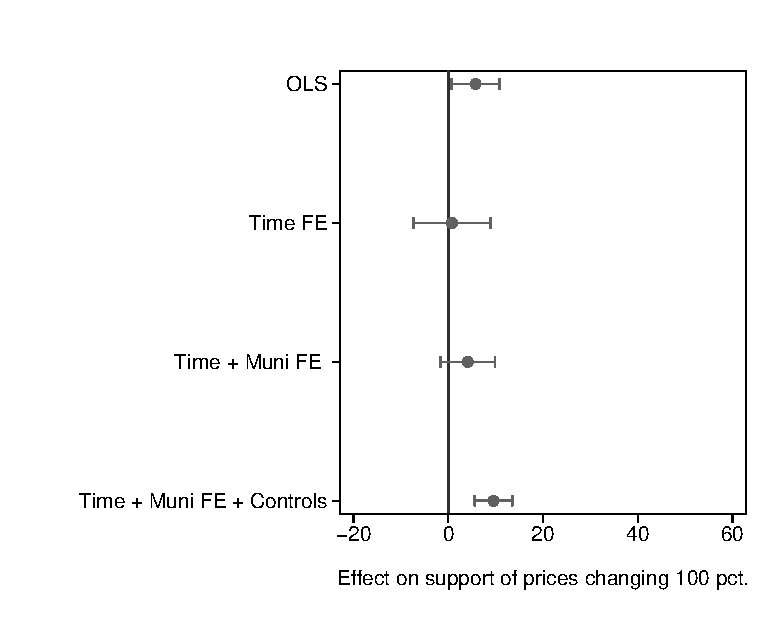
\includegraphics[width=1\textwidth]{pooled_effects.eps} 
		


   \column{0.5\textwidth} \pause
		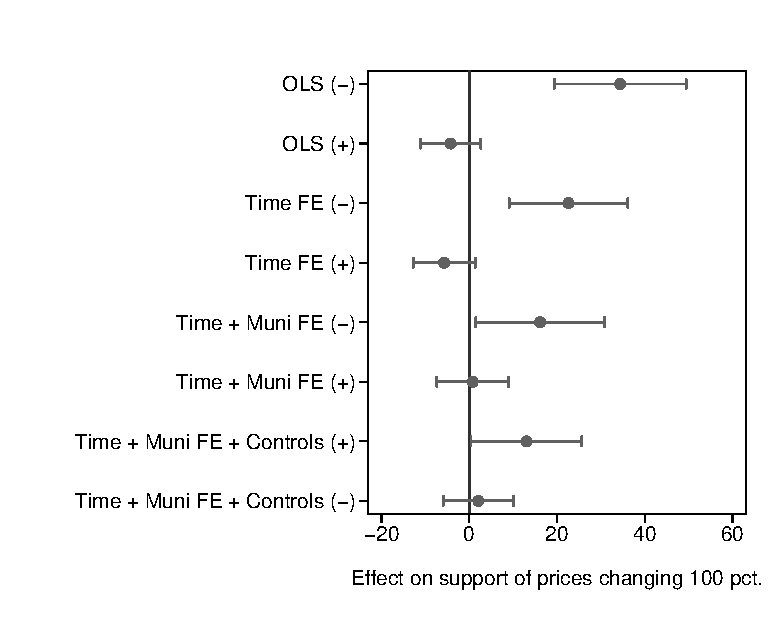
\includegraphics[width=1\textwidth]{posneg_effects.eps}
		\end{columns} 		\pause
		
	\centering{	\footnotesize{Controls: Unemployment, tax-level, violent crime, theft.}} 
\end{frame}	

\begin{frame}{Population based results}
	\begin{center}
			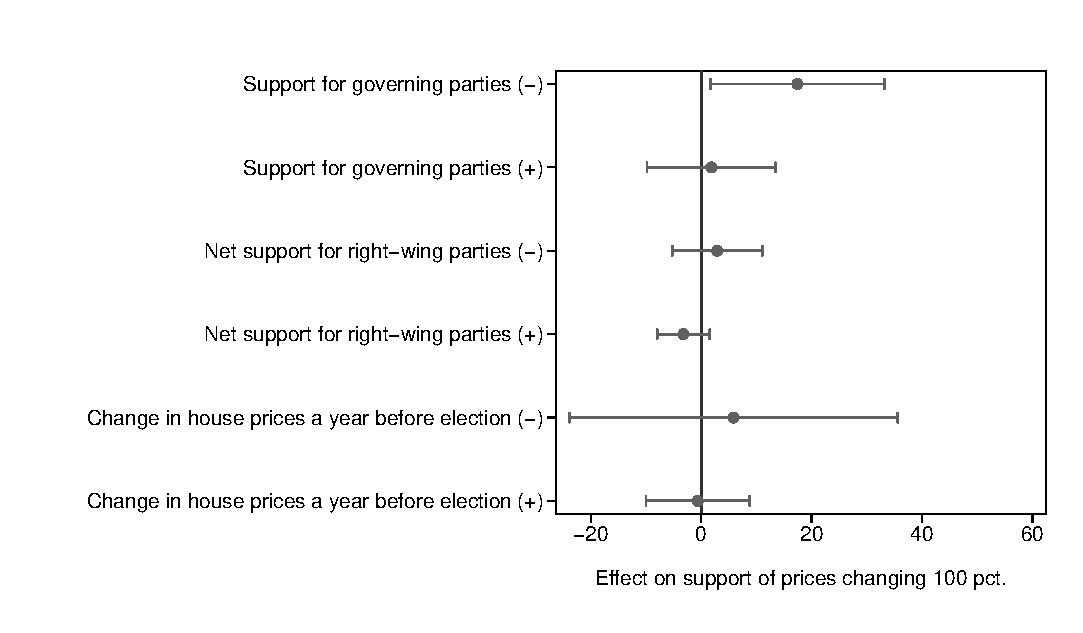
\includegraphics[width=0.6\textwidth]{robust.eps}
	\end{center}
\end{frame}	

\begin{frame}{Survey based results}
	
\end{frame}	

\section{Discussion}

	\begin{frame}{What is going on?}
	We have shown that falling - but not rising - house prices hurt incumbents in Denmark.
	
	\vspace{0.2in}
	
	Some questions we would like answered:
	\begin{itemize}
		\item is this convincing?
		\item what other analyses would you like to see?
		\item which interesting (theoretical and real world) implications do you think this has?
		\item do you think this is a case where personal economic grievances matter? 
	\end{itemize}	
		
	\end{frame}		



\end{document}